L'elettrochimica studia fenomeni elettrici dovuti al passaggio di corrente.

Visto che ragioniamo sempre in soluzioni acquose, il passaggio di corrente provoca dei fenomeni chimici. Può accadere anche il contrario: si genera energia elettrica tramite una reazione. Tratteremo entrambi i casi.

\vspace{0.2cm}Va da ricordare che energia elettrica significa flusso di elettroni.

Le reazioni che comportano scambi di elettroni sono le ossidoriduzioni, pertanto saremo interessati a questo tipo di reazioni.

Le redox a cui siamo interessati devono essere spontanee, perché sennò avverrebbe il contrario: facendo passare la corrente in soluzione indurremo reazioni redox. Dunque qualunque reazione redox spontanea è una sorgente di energia elettrica, ossia possiamo costruire una pila a partire da reazioni redox (tutte le pile comportano reazioni redox).

Consideriamo due esempi:

\begin{figure}[H]
    \centering
    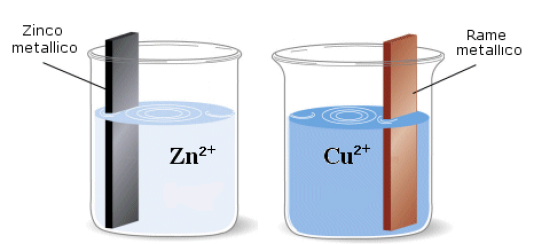
\includegraphics[width=10cm]{immagini/piastre_metalliche.png}
\end{figure}

Consideriamo dei beker conteneti acqua distillata in cui sono immersi un filo di zinco e un filo di rame.

In entrambi i casi stiamo immergendo in acqua un metallo, il quale inizia a liberare ioni. Ne segue che la lamina si caricherà di elettroni lasciati sulla lamina dagli ioni. Quindi la lamina, inizialmente neutra, immersa in acqua si carica negativamete e l'acqua distillata si arricchirà di ioni metallici. Quindi la soluzione inizialmente neutra si caricherà positivamente perché sta accettando cationi, mentre la lamina si caricherà negativamente perché ogni atomo che va in soluzione lascia elettroni su di essa


\begin{figure}[H]
    \centering
    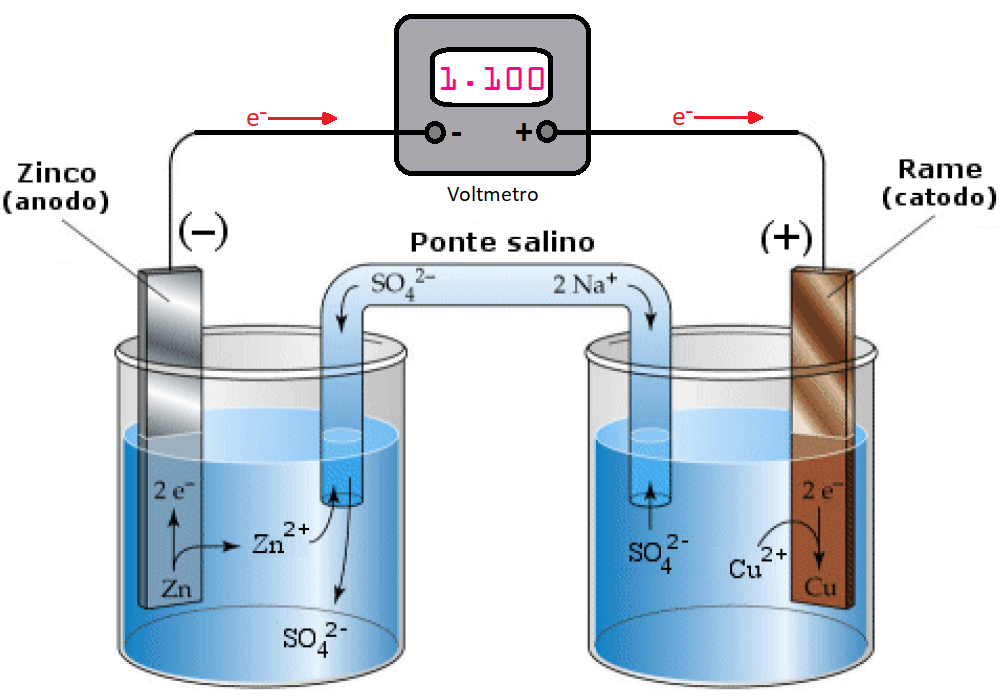
\includegraphics[width=12cm]{immagini/pila_di_Daniell.png}
\end{figure}
\begin{center}
    \hspace{0.3cm}\begin{tabular}{p{3.6cm}p{1.3cm}p{3.8cm}}
    \ce{Zn -> Zn^{2+} + 2 e^-} & & \ce{Cu^{2+} + 2e^- -> Cu}\\
    ossidazione, anodo & & riduzione, catodo
    \end{tabular}
\end{center}